\chapter{Resultados e Discussões}
\label{cap_3}

\section{Desenvolvimento do Protótipo e Softwares}

Os sistemas propostos tanto físico quanto softwares foram desenvolvidos de forma exitosa, os procedimentos para a implementação se deu a partir de uma pesquisa bibliográfica e criativa, tendo como resultado o protótipo, figura \ref{fig3:image_01}, e os softwares, figuras \ref{fig3:image_13_1}, \ref{fig3:image_14} e \ref{fig3:image_16}.


\section{Identificação de sistema aplicado ao Aeropêndulo}
\label{indentificacao}

Com os subsistemas desenvolvidos, foram realizados alguns testes para validá-los, assim, o primeiro teste aplicado ao conjunto se tratou da identificação de sistemas. Após a identificação realizou-se uma simulação de modo a comparar o sinal de saída real com o simulado, com o intuito de analisar a dinâmica do sistema identificado e poder comparar com o sistema real.

A partir da estrutura desenvolvido para o projeto é possível usá-lo para estudar diferentes aspectos na área de sistemas de controle, uma delas e a identificação de sistemas, para esse trabalho o método em questão foi usado para avaliar o correto funcionamento projeto. Desa forma, o trabalho \cite{tcc_klarissa_ufpa} foi usando como base teórica para implementar o método.


\subsubsection{Aplicação do Sinal PRBS na Entrada do Sistema}

O sinal PRBS aplicado a entrada do sistema em malha aberta foi gerado no microcontrolador e convertido em sinal PWM para ser aplicado a entrada do Driver L298N, subseção \ref{driver_l298n}, seus parâmetros foram definidos com uma amplitude de 0,3V, frequência fundamental de 0,4Hz e período de amostragem de 0,02 segundos, além disso, aplicou-se um offset de 1V (Ponto de operação), com isso, obteve-se o sinal PRBS de entrada mostrado na figura \ref{fig3:image_16}.


\begin{figure}[!h]
	\centering
	\caption{Sinal PRBS de entrada.}
	\efbox{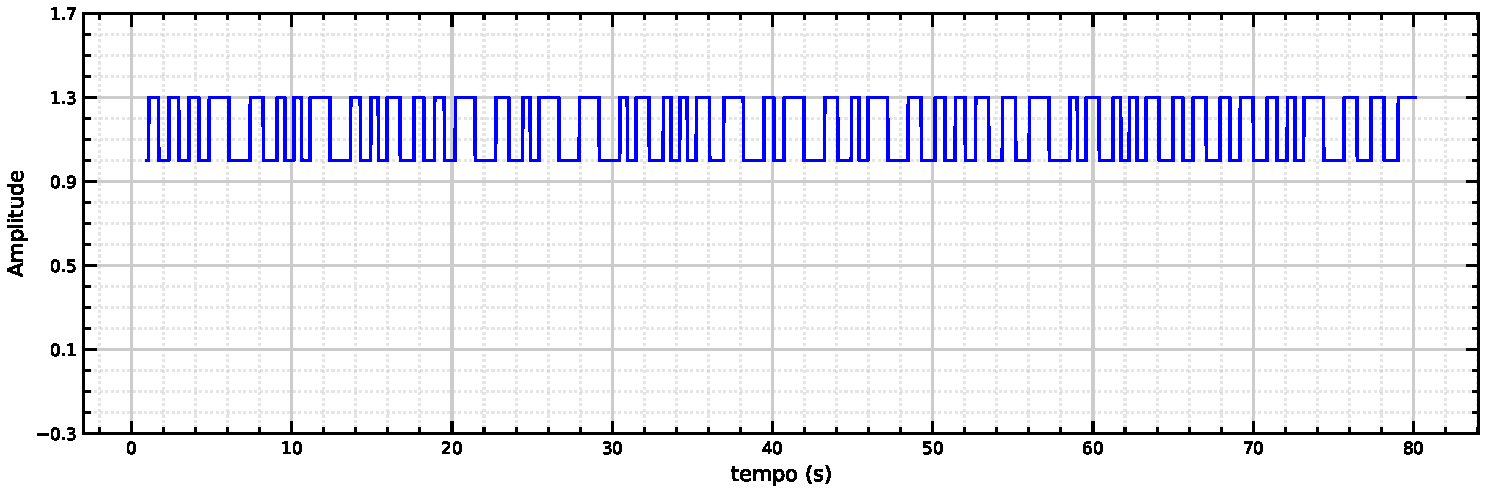
\includegraphics[width=1\textwidth]{Capitulos/3_1_resultados_discurcao/3_figuras/sinal_prbs_entrada_com_offset.pdf}}
	\caption*{Fonte: elaborado pelo autor (2023).}
	\label{fig3:image_18}
\end{figure}



\subsubsection{Sinal de Saída Gerado a Partir do Sinal PRBS de Entrada}

Para a obtenção do sinal de saída, que representa o ângulo do braço do aeropêndulo, foi empregado um método no qual um sinal PRBS foi aplicado à entrada do sistema. Para medir o ângulo, sinal de saída, utilizou-se um potenciômetro como sensor, cujas extremidades foram conectadas ao 3.3V e GND do ESP32. O terceiro fio do potenciômetro foi conectado a uma porta analógica do ESP32, permitindo, assim, a conversão da variação de tensão em valores angulares. A figura \ref{fig3:image_19} exibe o sinal de saída de um ensaio.

\begin{figure}[!h]
	\centering
	\caption{Sinal PRBS de saída.}
	\efbox{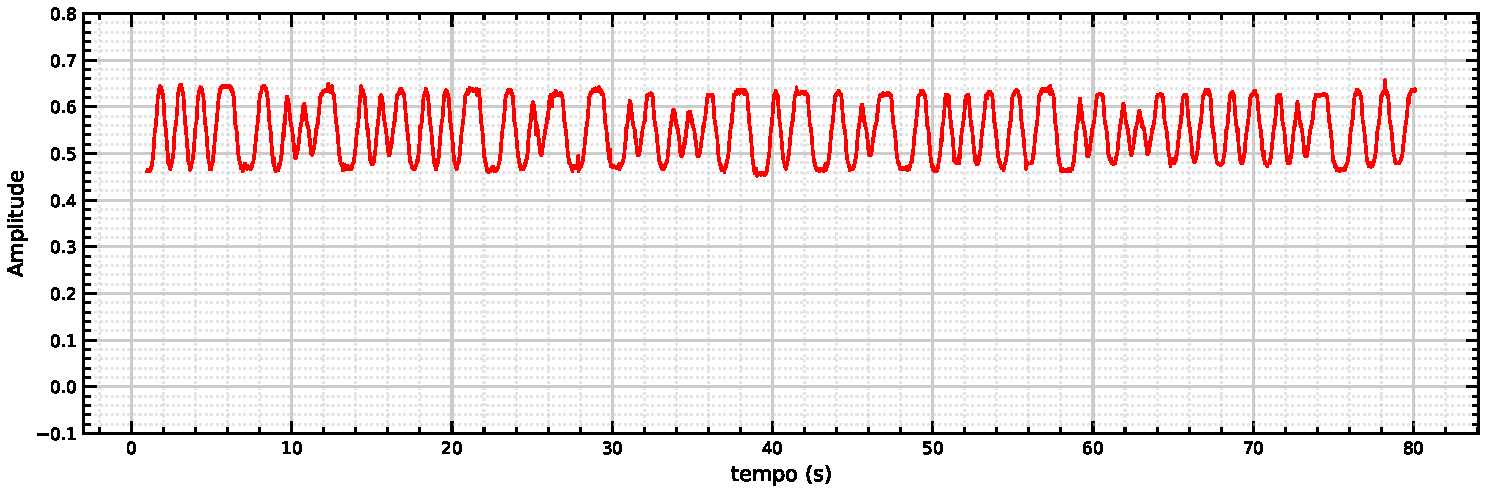
\includegraphics[width=1\textwidth]{Capitulos/3_1_resultados_discurcao/3_figuras/sinal_saida_com_offset.pdf}}
	\caption*{Fonte: elaborado pelo autor (2023).}
	\label{fig3:image_19}
\end{figure}

\subsection{Identificação Usando Mínimos Quadrados}


Para realizar a identificação de sistemas deve-se retirar os offsets tanto do sinal de entrada quanto para o de saída, com essa etapa realizada, deve-se separar dois conjuntos de dados para identificação e validação do modelo proposto, tanto para o sinal de entrada quanto para o de saída. Foi usando 60\% dos dados para identificação de 40\% para validação.

\subsubsection{Passos para realização da identificação}


\noindent\textit{Passo 1:} Obter dados Entrada/Saída do sistema;\\
\textit{Passo 2:} Dividir dados entre identificação e validação;\\
\textit{Passo 3:} Definir a Função de Transferência;\\
\textit{Passo 4:} Definir a matriz de regressão;\\
\textit{Passo 5:} Encontrar o vetor de coeficientes pela formulação de mínimos quadrados;\\
\textit{Passo 6:} Substituir os coeficientes na função de transferência escolhida anteriormente;\\
\textit{Passo 7:} Validar o modelo do sistema a partir de dados reais.\\

% O primeiro passo que deve ser realizado é escrever a estrutura da função de transferência proposta, dessa forma a equação \ref{eq3:eq1} foi a estrutura escolhida para modelar o sistema usando uma função de transferência de segunda ordem.

\subsubsection{Identificação Usando Função de Transferência Discreta de Segunda, Quinta e Décima Ordem}

Para realizar o cálculo numérico usando a base de dados do ensaio foi usando a linguagem de programação Python, que possui um conjunto de bibliotecas que facilita o implementação dos cálculos. Após obter os dados de ensaio, os passos seguintes foram desenvolvidos em um Script Python, sendo o primeiro passo a importação das bibliotecas, como mostra a célula de código abaixo.

\vspace{0.5cm}

\begin{lstlisting}[language=python, numbers=left, label=py3, caption={Importação das Bibliotecas usadas para identificação de sistemas.}]
import numpy as np 
import matplotlib.pyplot as plt
import pandas as pd
import control as ct
\end{lstlisting}

No segundo passo foi feito o carregamento dos dados de ensaio PRBS e realizada a separação entre dados de identificação e validação, para isso foi usado a biblioteca Pandas em conjunto com a biblioteca NumPy que possibilita carregar dados de diferentes formatos e manipulá-los, os dados de ensaio foram salvos em formato CSV (Comma-separated values), o código para realizar o carregamento dos dados e a separação é mostrado na célula de código abaixo.

\vspace{0.5cm}

\begin{lstlisting}[language=python, numbers=left, label=py4, caption={Carregando os dados do ensaio e realizando pré-processamento.}]
file = "caminho completo dos  dados/arquivo_9_9_2023_13_33_24.csv"
dados_malha_aberta_prbs = pd.read_csv(file, header=None, sep=',').values
dados_malha_aberta_prbs[0][0] = 0.0
dados_malha_aberta_prbs

# Variaveis contendo os dados de tempo, entrada e saida
tempo = np.array(dados_malha_aberta_prbs[:,7])
sinal_prbs_entrada  = np.array(dados_malha_aberta_prbs[:,6])
sinal_saida = np.array(dados_malha_aberta_prbs[:,2])

# Convertendo o sinal de Graus para Radianos
sinal_saida = np.squeeze(np.deg2rad(sinal_saida))
tempo = tempo - min(tempo)
\end{lstlisting}


Além disso, é necessário remover as primeiras amostras por conter o transitório do sistema e retirar os offsets dos sinais de entrada e saída, o que é feito na célula de código abaixo. A figura \ref{fig3:image_20} exibe os gráficos dos sinais de entrada/saída, podemos observar que os sinais estão centralizados em zero e não possui transitório no início do sinal.

\vspace{0.5cm}


\begin{lstlisting}[language=python, numbers=left, label=py3, caption={Centralizando os sinais de entrada e daída em zero.}]
u1 = sinal_prbs_entrada[50:] - np.mean(sinal_prbs_entrada[50:])
yout = sinal_saida[50:] - np.mean((sinal_saida[50:]))
t = tempo[50:]
\end{lstlisting}

\begin{figure}[!h]
	\centering
	\caption{Dados de identificação e validação do modelo.}
	\efbox{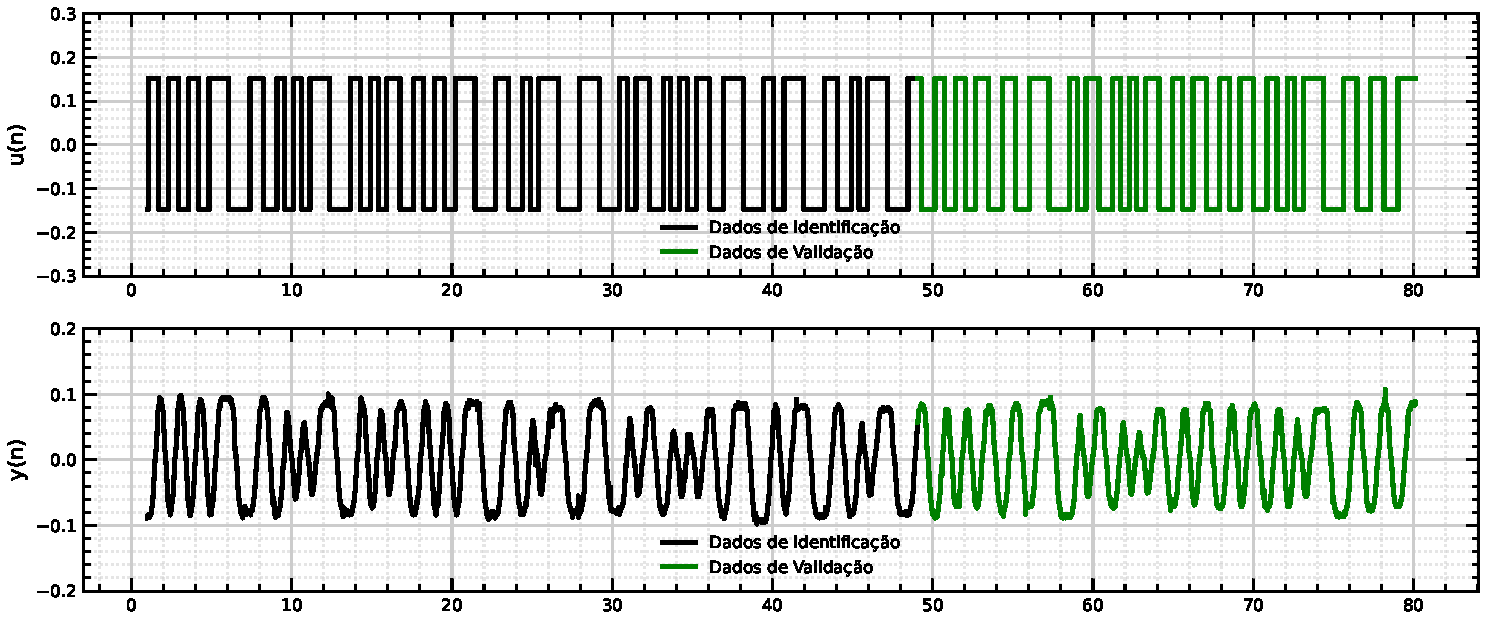
\includegraphics[width=1\textwidth]{Capitulos/3_1_resultados_discurcao/3_figuras/dados_traino_teste.pdf}}
	\caption*{Fonte: elaborado pelo autor (2023).}
	\label{fig3:image_20}
\end{figure}

Com os dados de ensaio pré-processados e prontos para aplicar a técnica de identificação, foi definida uma função de transferência discreta, essa função tem a finalidade de aproximar um modelo que satisfaça a dinâmica do aeropêndulo. Para um primeiro teste foi usada uma função de segunda ordem, como mostra a equação \ref{eq3:eq1}.

\begin{align}
    H(z) = \frac{b_1z^{-1}+b_2z^{-2}}
    {1+a_1z^{-1}+a_2z^{-2}} \label{eq3:eq1}
\end{align}

Para aplicar o método dos mínimos quadrados e obter os coeficientes da função de transferência de segunda ordem precisa-se ter as matrizes de regressão tando para os dados de entrada quanto para os de saída, o código abaixo cria o algorítimo necessário para se obter as matrizes a partir dos dados do ensaio.

\vspace{0.5cm}

\begin{lstlisting}[language=python, numbers=left, label=py3, caption={Estruturando os dados para aplicar o método dos mínimos quadrados.}]
# Matriz de regressao:
nb = 3; na = 2
ni = np.arange(na, Ni + na)
M = np.zeros((Ni, na + nb))

# Para regressores de y:
for l in np.arange(0, na):
  M[:, l] = yout[ni - l - 1]

# Para regressores de u:
for l in np.arange(0, nb):
  M[:, na + l] = u1[ni - l]

print(M.shape)
\end{lstlisting}

Com as matrizes de regressores definidas, foi realizada a aplicação do método dos mínimos quadrados, o que é exemplificado na célula de código abaixo, a biblioteca NumPy possibilita cálculos de álgebra matricial de forma rápida e simples.

\vspace{0.5cm}

\begin{lstlisting}[language=python, numbers=left, label=py3, caption={Método dos mínimos quadrados.}]
# Minimos quadrados
thetaA = np.linalg.inv(M.T @ M) @ M.T @ yout[ni]
thetaA
\end{lstlisting}

Para a função de transferência de segunda ordem escolhida, equação \ref{eq3:eq1}, em que possui dois coeficientes no numerador e 3 no denominador, dessa forma, os coeficientes obtidos ao aplicar o método de mínimos quadrados retorna em suas duas primeiras posições os coeficientes do numerador e o restante são os coeficientes do denominador, a partir dos coeficientes obtidos, pode-se definir a função de transferência discreta do sistema, isso é feito no Python usando a biblioteca Python-Control que permite realizar ensaios simulados a partir da função de transferência.

\vspace{0.5cm}

\begin{lstlisting}[language=python, numbers=left, label=py3, caption={Salvando os coeficientes em variáveis e obtendo a função de transferência.}]
a1, a2 = thetaA[:2]
b0, b1, b2 = thetaA[2:]

Ba = [b0 , b1, b2]
Aa = [1, -a1, -a2]

Hz = ct.tf(Ba, Aa, Ts)
\end{lstlisting}

Função de transferência discreta, \ref{eq3:eq2}, com os coeficientes obtidos a partir do método de mínimos quadrados, o período de amostragem é $dt = 0,019$  segundos.

\begin{align}
Hz = \frac{-0.002602 z^2 + 0.004962 z + 0.0163}{z^2 - 1.176 z + 0.1849} \label{eq3:eq2}
\end{align}


Para validar o modelo encontrado é preciso testar a função de transferência discreta usando os dados de entrada do ensaio real, com isso obtém-se os dados de saída da simulação, esse dado pode ser comparado com a saída do sistema real, caso ambos os gráficos aproximem suas dinâmicas pode-se concluir que o modelo corresponde com o sistema real, caso contrário é preciso definir uma nova função de transferência e realizar novamente o teste de validação.

A biblioteca Python-control possibilita simular a dinâmica de um sistema a partir da sua função de transferência discreta, podendo receber como argumento um vetor de entradas, como mostrado a célula de código abaixo.

\vspace{0.5cm}

\begin{lstlisting}[language=python, numbers=left, label=py3, caption={Obtendo a resposta forçada da função de transferência obtida.}]
_, yp = ct.forced_response(Hz, U=u1)
\end{lstlisting}

Ao plotar os gráficos de saída real e simulada tem-se como resultado a figura \ref{fig3:image_21}, é possível observar que a saída da simulação não corresponde de forma aceitável com a dinâmica do sinal de saída do sistema real, ou seja, o modelo não foi robusto o suficiente para identificar o sistema em questão.

\begin{figure}[!h]
	\centering
	\caption{Validação do modelo de segundo grau.}
	\efbox{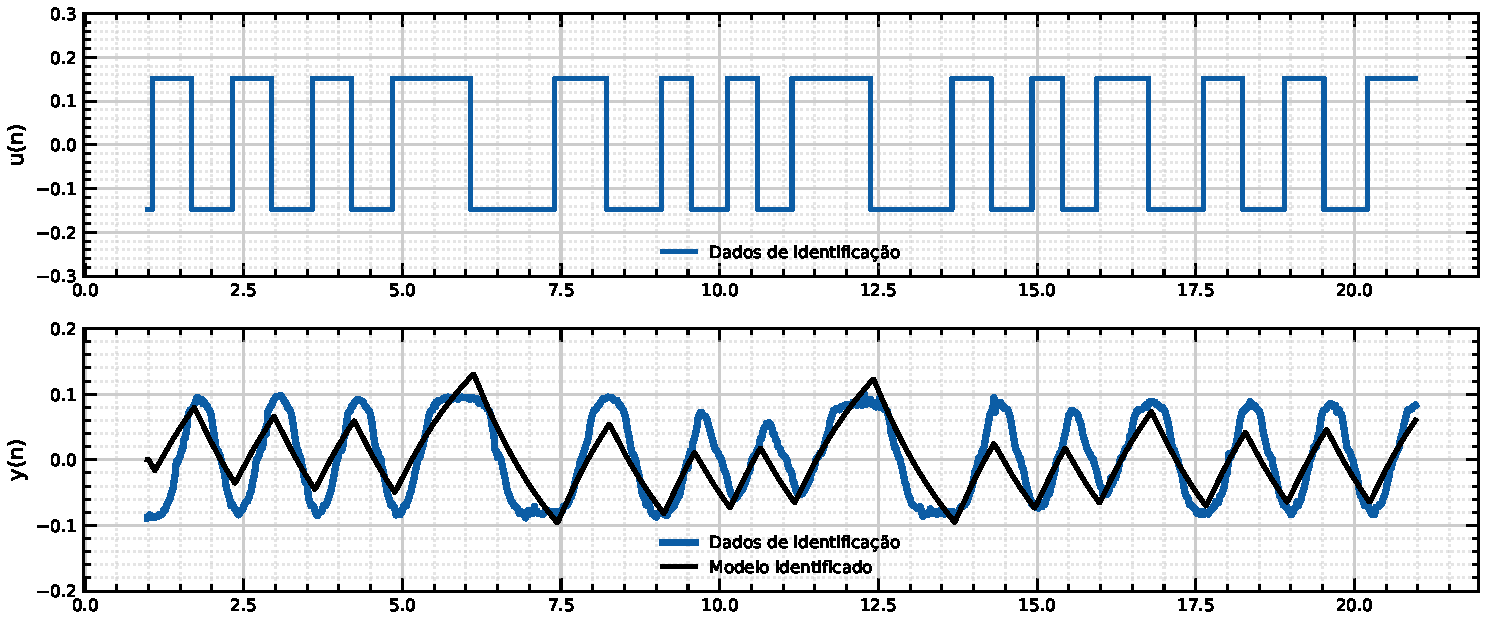
\includegraphics[width=1\textwidth]{Capitulos/3_1_resultados_discurcao/3_figuras/validacao_model_2grau.pdf}}
	\caption*{Fonte: elaborado pelo autor (2023).}
	\label{fig3:image_21}
\end{figure}

A partir de uma análise qualitativa, pode-se supor que o grau da função de transferência discreta escolhida não consegue aproximar a dinâmica real do aeropêndulo, dessa forma, foi realizado alguns testes e identificado que uma função de transferência discreta de décima ordem, equação \ref{eq3:eq3}, aproxima de forma aceitável o sistema real.  Com numerador dados pelos por, $[b_1z^{-1}+b_2z^{-2}+b_2z^{-3}+b_2z^{-4}]$ e denominador dado pelos, $[1+a_1z^{-1}+a_2z^{-2}+a_2z^{-3}+a_2z^{-4}+a_2z^{-5}+a_2z^{-6}+a_2z^{-7}+a_2z^{-8}+a_2z^{-9}+a_2z^{-10}]$.


\begin{align}
H(z) = \frac{numerador}{denominador}\label{eq3:eq3}
\end{align}


Assim, foi ajustado o algorítimo para identificar o sistema a partir da estrutura da equação \ref{eq3:eq3}, o código abaixo gera as matrizes tanto para os regressores de entrada quanto para o de saída. 

\vspace{0.5cm}

\begin{lstlisting}[language=python, numbers=left, label=py3, caption={Estruturando os dados para aplicar o método dos mínimos quadrados.}]
# Matriz de regressao:
nb = 4
na = 10
ni = np.arange(na, Ni + na)
M = np.zeros((Ni, na + nb))

# Para regressores de y:
for l in np.arange(0, na):
  M[:, l] = yout[ni - l - 1]

# Para regressores de u:
for l in np.arange(0, nb):
  M[:,na+l] = u1[ni-l]

print(M.shape)
\end{lstlisting}


Com as matrizes de regressores ajustada para um sistema de décima ordem, foi realizada a aplicação do método dos mínimos quadrados.

\vspace{0.5cm}

\begin{lstlisting}[language=python, numbers=left, label=py3, caption={Método dos mínimos quadrados.}]
# Minimos quadrados
thetaA = np.linalg.inv(M.T @ M) @ M.T @ yout[ni]
thetaA
\end{lstlisting}

A equação \ref{eq3:eq3} possui 4 coeficientes no numerador e 10 no denominador, dessa forma, as quatro primeiras posições da variável  \textbf{thetaA} corresponde aos coeficientes do numerador e o restante aos coeficientes do denominador, a célula de código abaixo define a função de transferência usando a estrutura da equação \ref{eq3:eq3} e os coeficientes obtidos.

\vspace{0.5cm}

\begin{lstlisting}[language=python, numbers=left, label=py3, caption={Salvando os coeficientes em variáveis e obtendo a função de transferência.}]
a1, a2, a3, a4, a5, a6, a7, a8, a9, a10 = thetaA[:10]
b0, b1, b2, b3 = thetaA[10:]

Ba = [b0 , b1, b2, b3]
Aa = [1, -a1, -a2, -a3, -a4, -a5, -a6, -a7, -a8, -a9, -a10]

Hz = ct.tf(Ba, Aa, Ts)
\end{lstlisting}

Assim, obtém-se a função de transferência discreta, equação \ref{eq3:eq4}, com os valores encontrado a partir do método de mínimos quadrados, com período de amostragem de $dt = 0,02$ segundos. Com numerador dados pelos valores, $[-0.0029 z^3 + 0.0023z^2 + 0.0016 z + 0.0097]$ e denominador dado pelos valores, $[z^{10} - 0.9 z^9 - 0.3 z^8 - 0.014 z^7 + 0.13 z^6 + 0.15 z^5 + 0.012 z^4 - 0.05 z^3 - 0.12 z^2 - 0.02 z + 0.15]$.

\begin{align}
Hz = \frac{numerador}{denominador} \label{eq3:eq4}
\end{align}

Por fim, realizou-se novamente a simulação do modelo encontrado, com o propósito de compará-lo aos dados de saída obtidos durante o ensaio do sistema real, a célula de código abaixo implementa a simulação.

\vspace{0.5cm}

\begin{lstlisting}[language=python, numbers=left, label=py3, caption={Obtendo a resposta forçada da função de transferência obtida.}]
_, yp = ct.forced_response(Hz, U=u1)
\end{lstlisting}


\begin{figure}[!h]
	\centering
	\caption{Validação do modelo de segundo grau.}
	\efbox{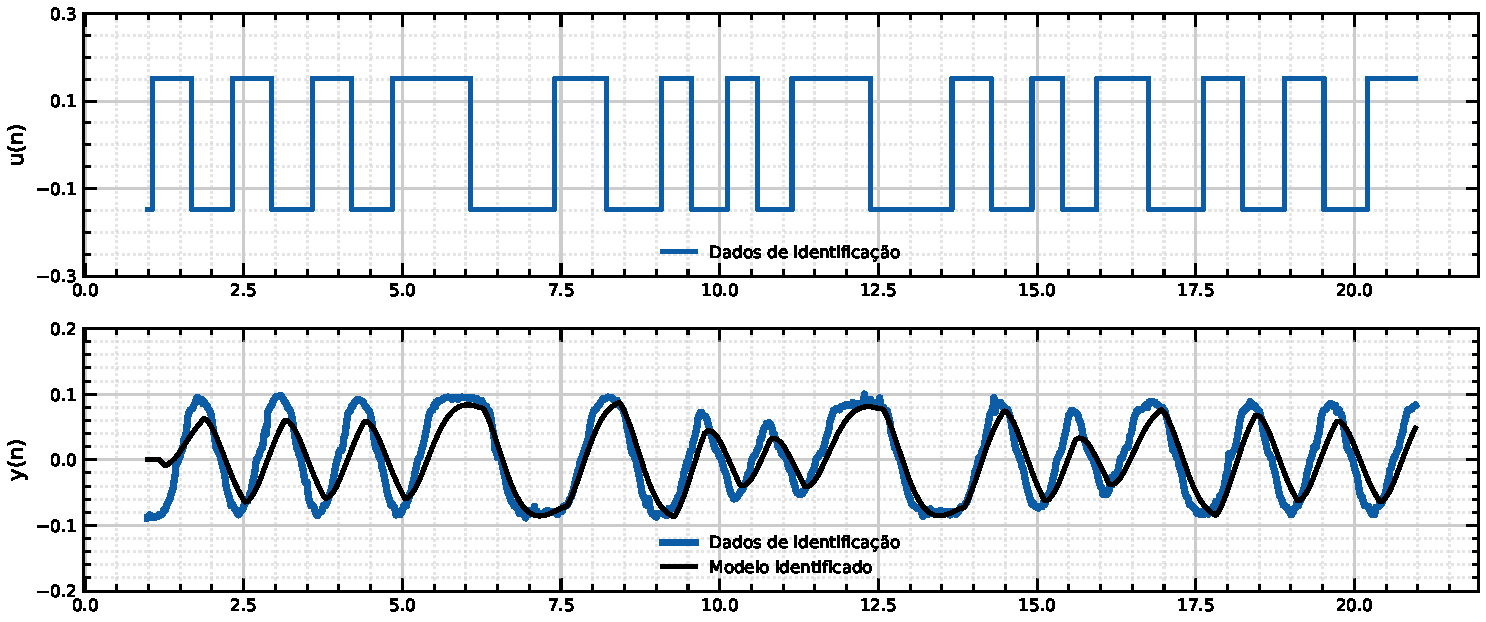
\includegraphics[width=1\textwidth]{Capitulos/3_1_resultados_discurcao/3_figuras/validacao_model_10grau.pdf}}
	\caption*{Fonte: elaborado pelo autor (2023).}
	\label{fig3:image_22}
\end{figure}


A partir de uma análise qualitativa entre o sinal de saída real e o simulado, figura \ref{fig3:image_22}, pode-se concluir que o modelo proposto a partir do método de mínimos quadrados teve exito, no entanto, ao modelar sistemas reais sempre haverá erro, isso por conta da não linearidade dos componentes físicos: sensores, atuadores e do próprio sistema, sedo assim, o modelo obtido é apenas uma aproximação do sistema real. %, para aplicar uma análise quantitativa, pode-se recorrer a alguns métodos de avaliação do modelo, para este exemplo, foi usado o Erro Quadrático Médio (EQM), equação \ref{eq3:eq4}.


\section{Ensaio em Malha Fechada com Controlador PID}
\label{malha_fechada}

Com a arquitetura desenvolvida para o firmware do microcontrolador é possível aplicar diferentes controladores, bastando implementá-lo no formato de uma biblioteca e chamá-la no código principal do firmware, passando como parâmetro o erro que é calculado subtraindo da referência o valor lido na saída do sistema, isso permite maior flexibilidade ao pesquisador, que pode projetar diferentes controladores e realizar seus testes sem que seja necessário sobrescrever o código de implementação do sistema de controle, ou seja, a equação do controlador.

Com  proposito de testar o sistema em malha fechada, foi desenvolvido um controlador PID simples, tendo apenas um requisito, erro nulo para o sinal degrau. A figura \ref{fig3:image_23} exibe o diagrama do controlador proposto.% A equação \ref{eq3:eq5} exibe a estrutura do controlado já com os ganhos.


\begin{figure}[!h]
	\centering
	\caption{Sistema em Malha Fechada com Controlador PID.}
	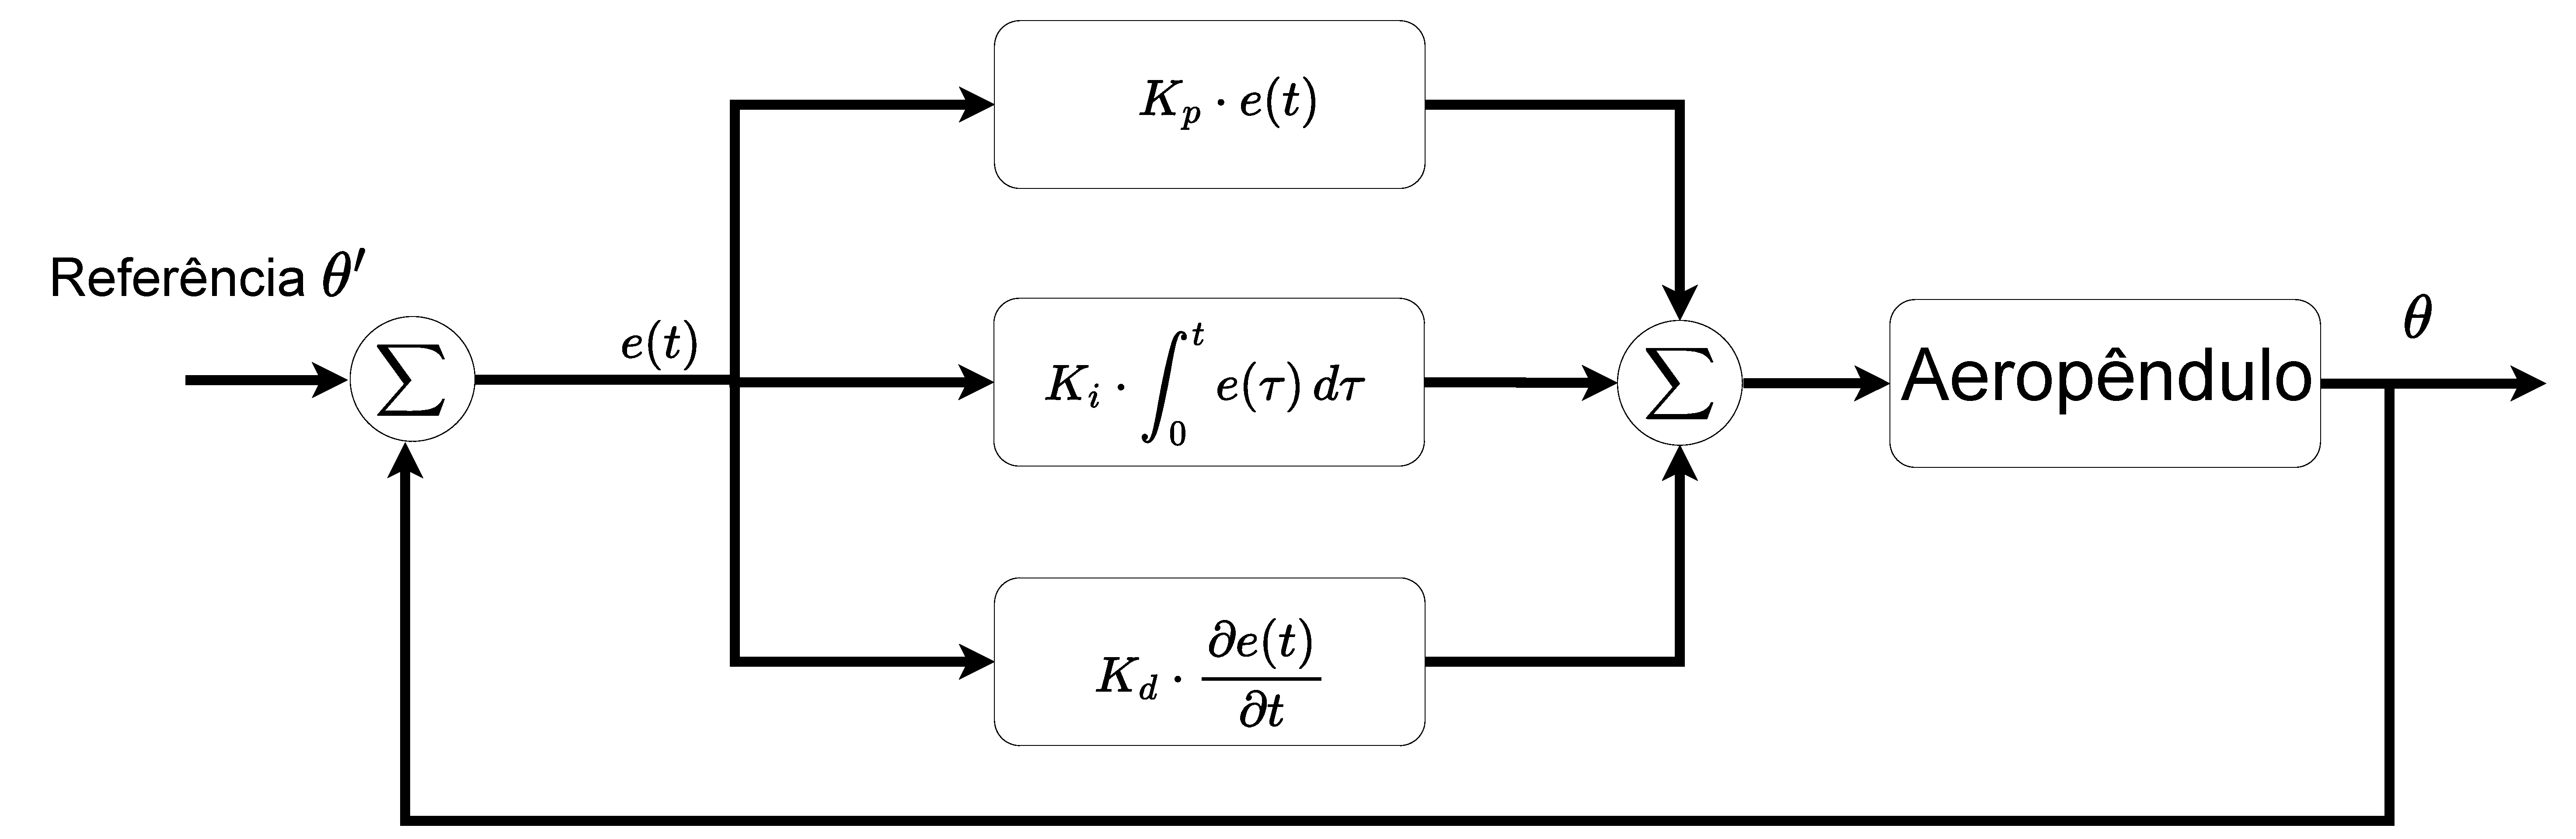
\includegraphics[width=1\textwidth]{Capitulos/3_1_resultados_discurcao/3_figuras/estrutura_pid.pdf}
	\caption*{Fonte: elaborado pelo autor (2023).}
	\label{fig3:image_23}
\end{figure}


No contexto da validação do sistema em malha fechada, optou-se por uma abordagem simplificada para a sintonia do controlador PID. Este método baseou-se na técnica de tentativa e erro. Após uma série de experimentos, determinou-se valores para os coeficientes do controlador, que foram os seguintes: $K_p=0,02$, $K_i=0,055$ e $K_d=0,35$.

% \begin{align}
% \frac{-0.0029 z^3 + 0.0023z^2 + 0.0016 z + 0.0097}{z^{10} - 0.9 z^9 - 0.3 z^8 - 0.014 z^7 + 0.13 z^6 + 0.15 z^5 + 0.012 z^4 - 0.05 z^3 - 0.12 z^2 - 0.02 z + 0.15}\quad dt = 0.02\label{eq3:eq5}
% \end{align}


\subsection{Onda Quadrada}

Ao inicializar a interface é possível escolher a opção de malha fechada, com isso a interface envia um comando para o microcontrolador que fecha a malha e aplica o sinal de controle na entrada do sistema, dessa forma, o aeropêndulo rasteia o sinal de referência escolhido, para o primeiro teste foi escolhido como sinal de referência uma onda quadrada com os seguintes parâmetros, frequência de 0,5 Hz, Amplitude 15° e offset de 1V. A figura \ref{fig3:image_24}, permite visualizar os sinais de referência e saída, ao analisá-los pode-se observar que o sinal de saída rasteia o sinal de referência. Além disso, observa-se que o sistema possui um transitório nas extremidades do sinal de onda quadrada, isso pode ser analisado a partir do sinal de erro que aumenta as extremidades do sinal de referência.

O gêmeo digital consome em tempo real o sinal angular do sistema real capturado através do potenciômetro, com isso é possível visualizar de uma forma gráfica a dinâmica do sistema real.

\begin{figure}[!h]
	\centering
	\caption{Gráficos dos Estados do Aeropêndulo com Controlador PID.}
	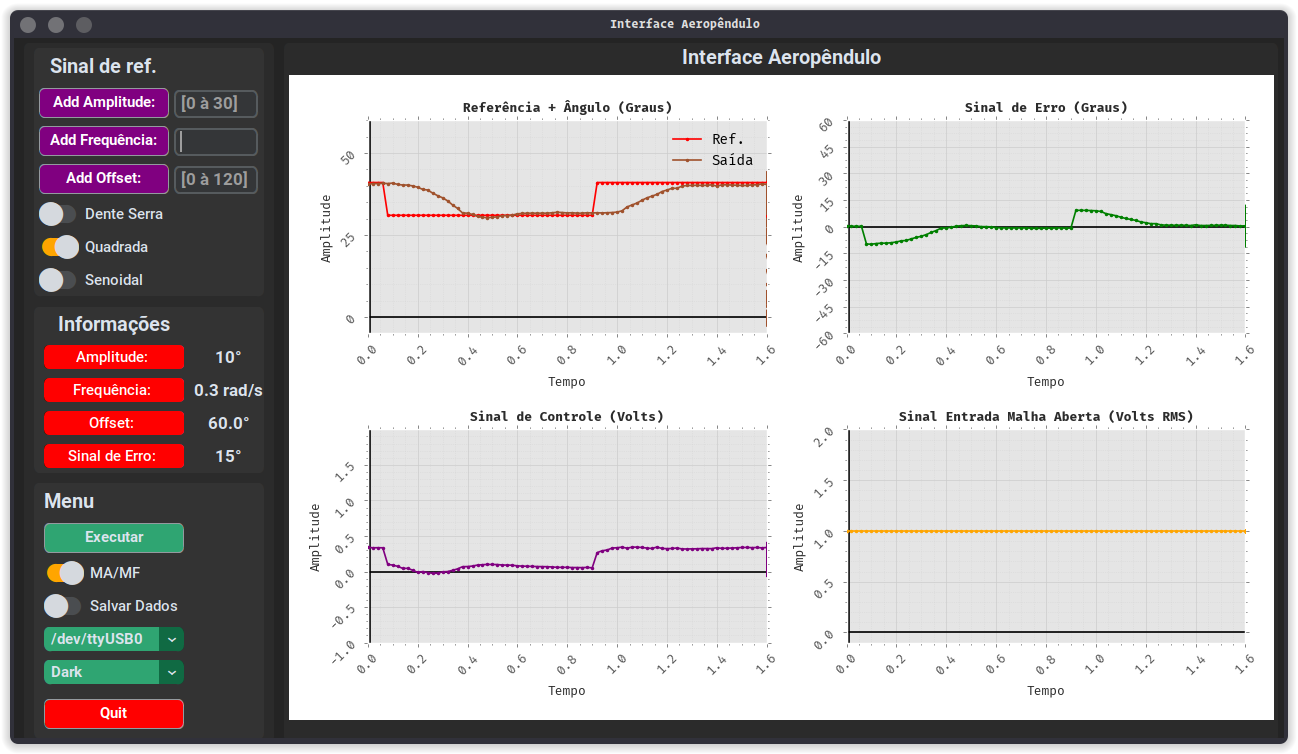
\includegraphics[width=0.9\textwidth]{Capitulos/3_1_resultados_discurcao/3_figuras/mf_gui_d1.png}
	\caption*{Fonte: elaborado pelo autor (2023).}
	\label{fig3:image_24}
\end{figure}


\begin{figure}[!h]
	\centering
	\caption{Gêmeo Digital com Controlador PID.}
	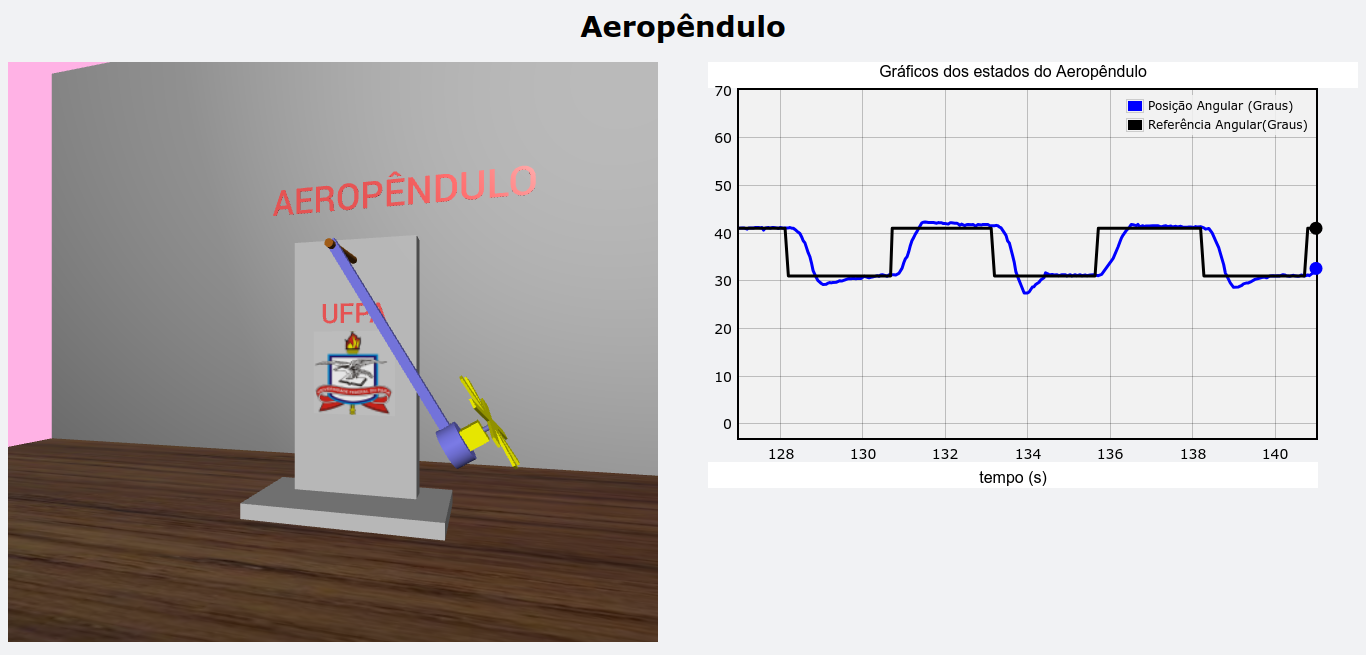
\includegraphics[width=0.9\textwidth]{Capitulos/3_1_resultados_discurcao/3_figuras/mf_gemeo_d1.png}
	\caption*{Fonte: elaborado pelo autor (2023).}
	\label{fig3:image_25}
\end{figure}


\subsection{Onda Dente de Serra}

Com o sinal de referência sendo uma onda dente de serra, pode-se observar que o controlador consegue rastreá-lo, tendo assim como no sinal degrau, um transitório nas extremidades.

\begin{figure}[!h]
	\centering
	\caption{Sistema em Malha Fechada com Controlador PID.}
	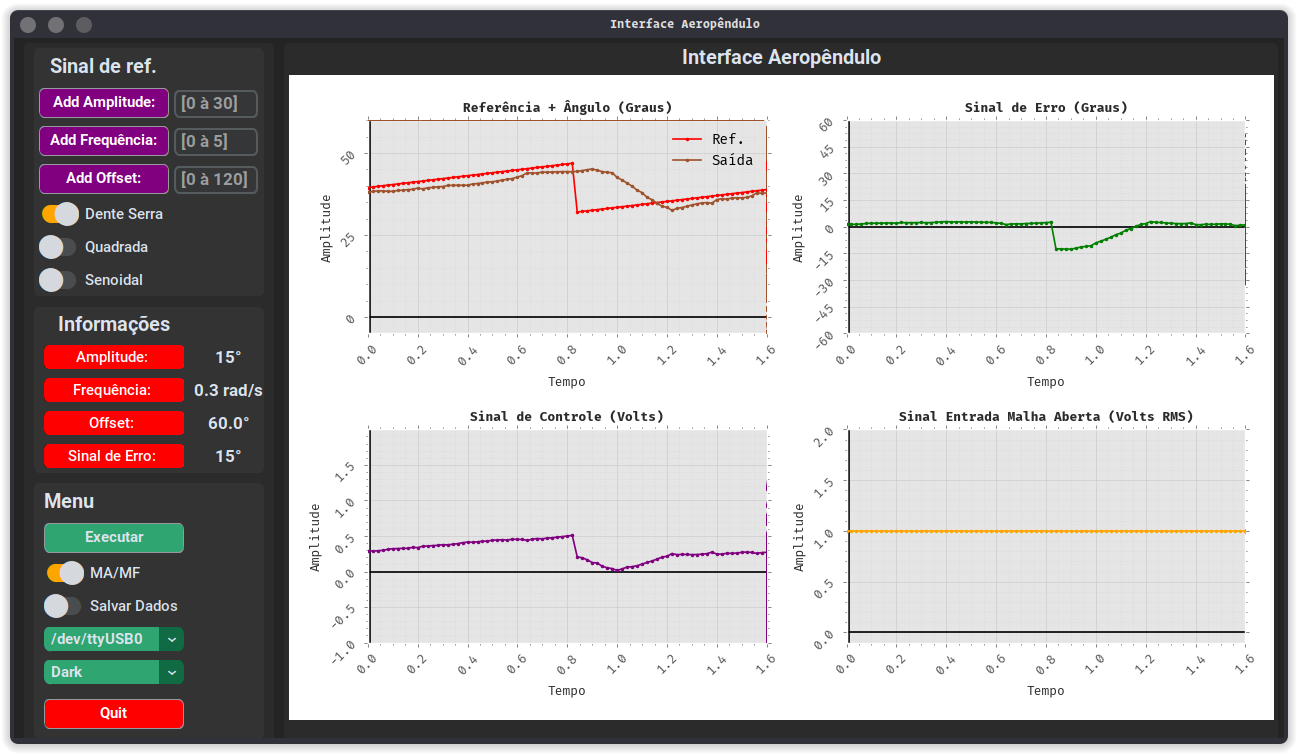
\includegraphics[width=0.9\textwidth]{Capitulos/3_1_resultados_discurcao/3_figuras/mf_gui_den1.png}
	\caption*{Fonte: elaborado pelo autor (2023).}
	\label{fig3:image_26}
\end{figure}


\begin{figure}[!h]
	\centering
	\caption{Gêmeo Digital consumindo os dados em tempo real do protótipo em Malha Fechada com Controlador PID.}
	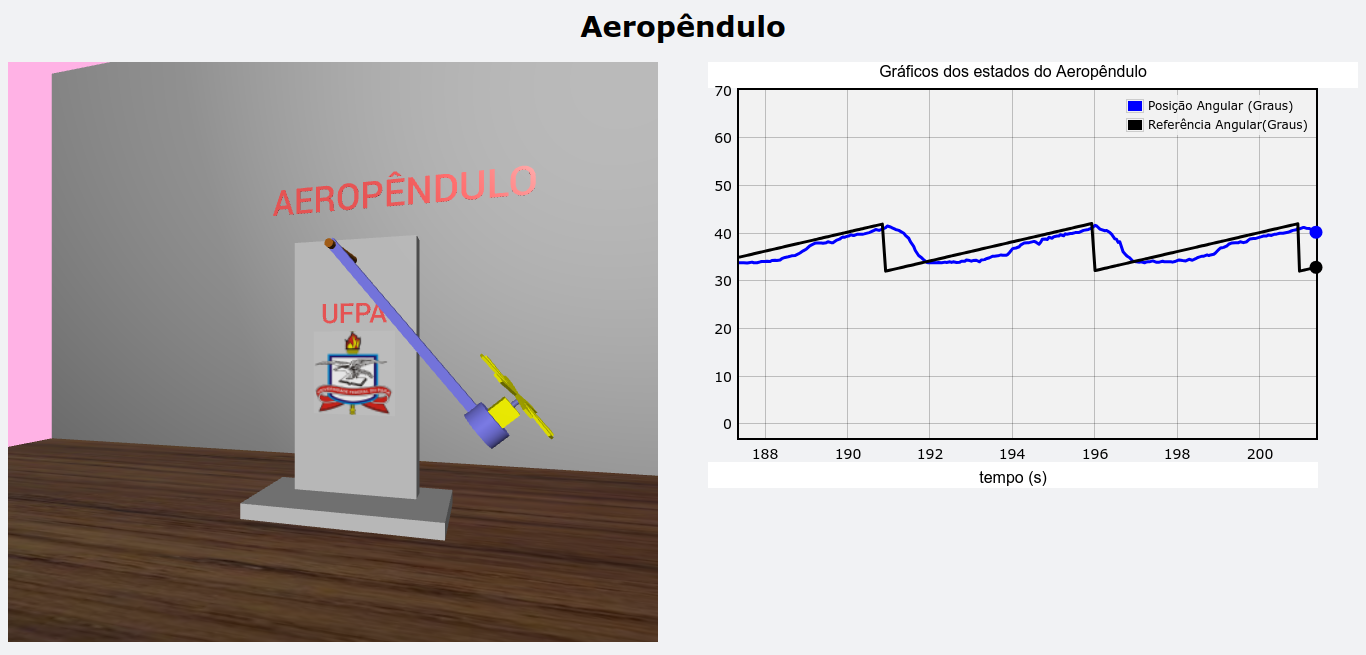
\includegraphics[width=0.9\textwidth]{Capitulos/3_1_resultados_discurcao/3_figuras/mf_gem_den1.png}
	\caption*{Fonte: elaborado pelo autor (2023).}
	\label{fig3:image_27}
\end{figure}


